%%%%%%%%%%%%%%%%%%%%%%%%%%%%%%%%%%%%%%%%%%%%%%%%%%%%%%%%%%%%%%%%%%%%%%%%%%%%%%%
\chapter{Lei de Hooke}
\label{Chap:ExpLeiDeHooke}
%%%%%%%%%%%%%%%%%%%%%%%%%%%%%%%%%%%%%%%%%%%%%%%%%%%%%%%%%%%%%%%%%%%%%%%%%%%%%%%

\begin{fullwidth}\it
	Realizaremos um experimento em que submeteremos uma mola a forças com intensidades diferentes, observando as distensões correspondentes. Procuramos assim observar experimentalmente a Lei de Hooke -- que afirma que as distensões são diretamente proporcionais à intensidade da força aplicada --. Utilizaremos os seguintes conceitos: medidas, algarismos significativos, gráficos, erros de escala e propagados, e regressão linear.
\end{fullwidth}

%%%%%%%%%%%%%%%%%%%%%%%%%%%%%%%%%%%%%%%%%%%%%%%%%%%%%%%%%%%%%%%%%%%%%%%%%%%%%%%
\section{Lei de Hooke}
%%%%%%%%%%%%%%%%%%%%%%%%%%%%%%%%%%%%%%%%%%%%%%%%%%%%%%%%%%%%%%%%%%%%%%%%%%%%%%%

Se usarmos uma corda para pendurar uma caixa ao teto de uma sala e passarmos a colocar objetos em tal caixa, não temos nenhuma indicação visual de qual é a força exercida pela corda. Poderíamos aferir a massa de cada objeto antes de os colocar na caixa e assim teríamos condições de saber qual a força exercida pela corda.

Para uma mola, se realizássemos o mesmo procedimento, verificaríamos uma \emph{distensão} gradual da mola. Fazendo um \emph{diagrama de corpo livre} (Figura~\ref{DiagramaCorpoLivre}), sabendo ainda que a aceleração do sistema é zero em uma condição de equilíbrio, concluímos que a força exercida pela mola sobre a caixa é igual em módulo e tem direção contrária à força peso da caixa (juntamente com sua carga):
\begin{equation}
	\vec{F}_e = -\vec{P}.
\end{equation}

\begin{marginfigure}
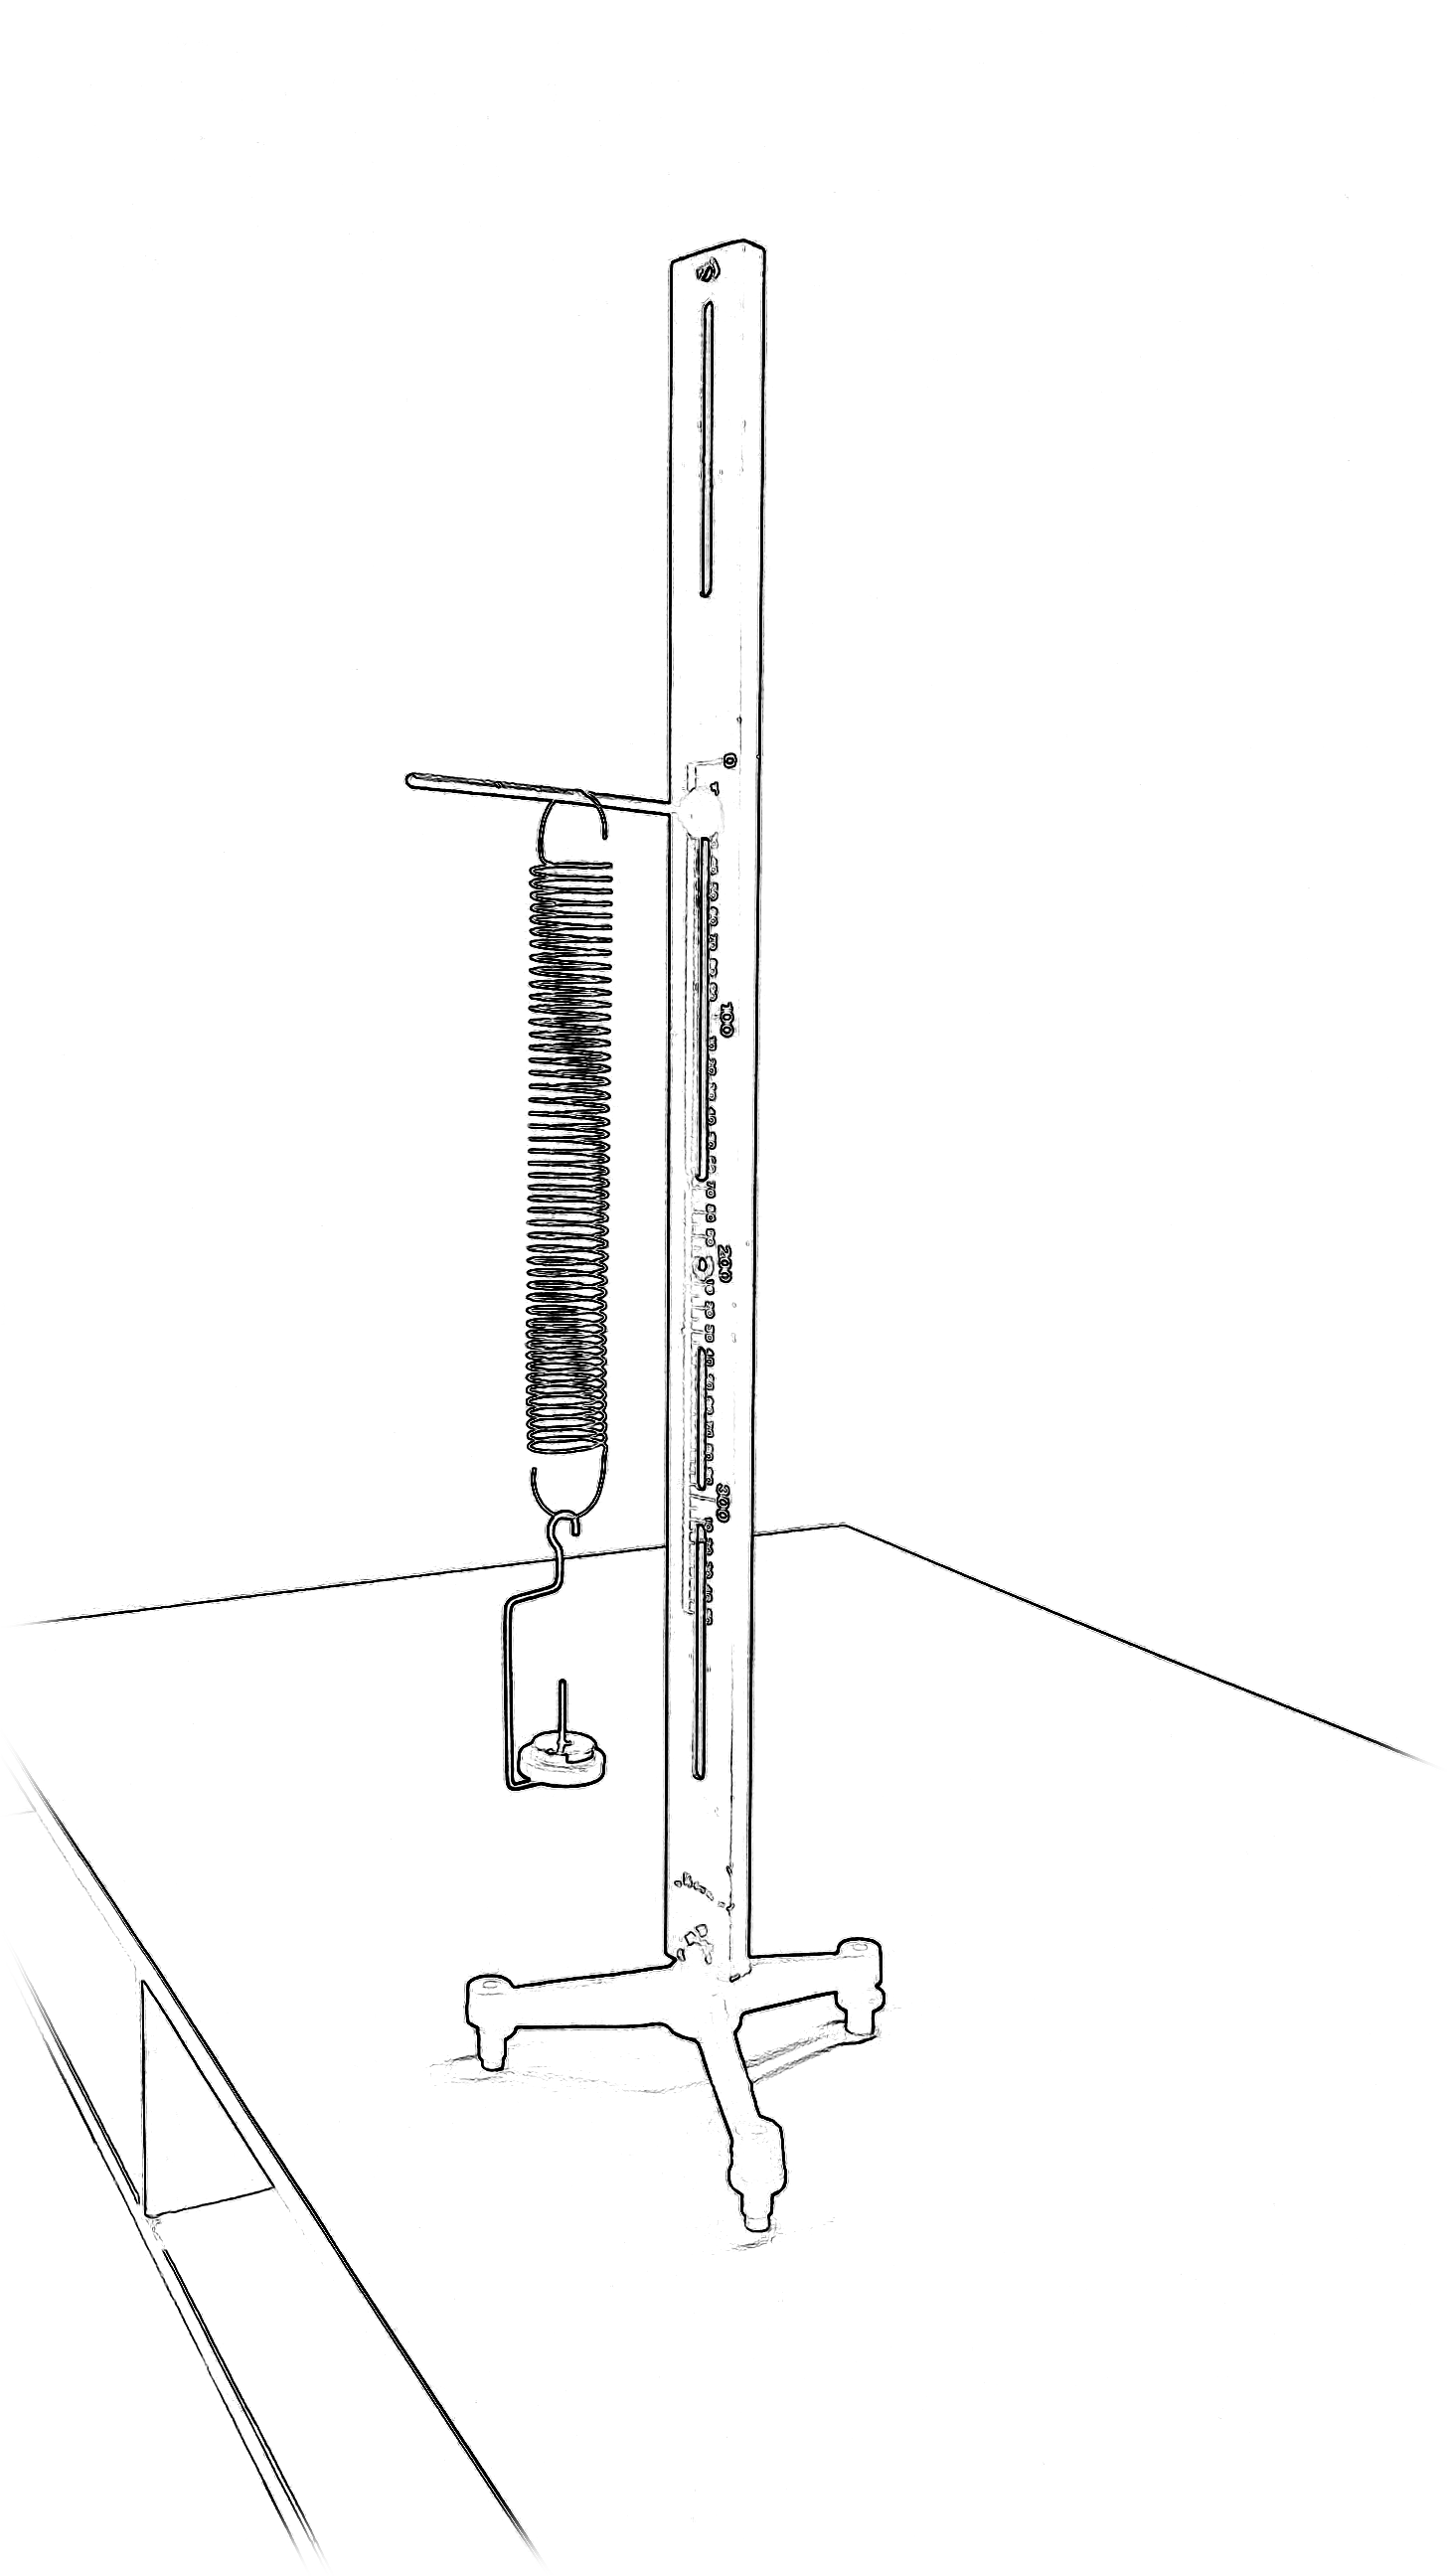
\includegraphics[width=\textwidth]{Ilustrations/Hooke.png}
\caption{Aparato para a verificação da distensão de um mola em função da massa por ela suportada.}
\end{marginfigure}

Verificando ainda a distensão da mola, podemos relacionar uma maior distensão a uma carga maior na caixa, isto é, quanto maior a força peso dos objetos pendurados na mola, maior a distensão. Experimentalmente, verifica-se que a relação entre o peso aplicado à mola e sua distensão são \emph{diretamente proporcionais}:
\begin{equation}
	\Delta x \propto P.
\end{equation}

Podemos então escrever para a \textbf{força elástica} $F_e$
\begin{equation}
	\vec{F}_e \propto -\vec{d},
\end{equation}
%
onde $\vec{d}$ representa o deslocamento $\Delta x$ em módulo e direção. Podemos escrever a relação acima como uma igualdade introduzindo uma constante de proporcionalidade $k$:
\begin{equation}
	\vec{F}_e = -k \vec{d}.
\end{equation}

\begin{marginfigure}
\centering
\begin{tikzpicture}[>=Stealth]
	\draw[fill] (0,0) circle[radius = 0.1];
	\draw[->] (0,0) -- node[right]{$\vec{F}_e$}(0,1);
	\draw[->] (0,0) -- node[right]{$\vec{P}$}(0,-1);
\end{tikzpicture}
\caption{Diagrama de corpo livre para o corpo sustentado pela mola quando em equilíbrio.}
\label{DiagramaCorpoLivre}
\end{marginfigure}

O resultado acima é conhecido como \emph{Lei de Hooke}, em homenagem ao físico inglês Robert Hooke, que o enunciou em 1660. Tal relação, no entanto, só é válida para um intervalo de distensões da mola. As distensões dentro deste limite são denominadas \emph{elásticas} e não deformam a mola permanentemente, caso contrário ao das distensões \emph{plásticas}. Apesar de a validade da Lei de Hooke ser limitada, ela é o modelo mais comum ao se analisar a resposta de um meio a uma deformação e pode ser utilizada como uma primeira aproximação mesmo para casos mais complexos.

%%%%%%%%%%%%%%%%%%%%%%%%%%%%%%%%%%%%%%%%%%%%%
%\subsection{Se necessário, usar subsections}
%%%%%%%%%%%%%%%%%%%%%%%%%%%%%%%%%%%%%%%%%%%%%

%%%%%%%%%%%%%%%%%%%%%%%%%%%%%%%%%%%%%%%%%%%%%%%%%%%%%%%%%%%%%%%%%%%%%%%%%%%%%%%
\section{Experimento}
%%%%%%%%%%%%%%%%%%%%%%%%%%%%%%%%%%%%%%%%%%%%%%%%%%%%%%%%%%%%%%%%%%%%%%%%%%%%%%%

%%%%%%%%%%%%%%%%%%%%%%
\subsection{Objetivos}
%%%%%%%%%%%%%%%%%%%%%%

\begin{itemize}
     \item Verificar a lineariedade da distensão de uma mola em resposta à força peso dos objetos pendurados nela.
	 \item Relacionar as variáveis da Lei de Hooke às da equação da reta $y = A + Bx$.
     \item Calcular a constante $k$ da mola;
     \item Elaborar um gráfico $\Delta x \times P$ dos pontos experimentais e adicionar a ele a reta calculada através da regressão linear;
\end{itemize}

%%%%%%%%%%%%%%%%%%%%%%%%%%%%%%%%%%%%%%%%%%%%%%%%%%%%%%%%%%%%%%%%%%%%%%%%%%%%%%%
\section{Material Necessário}
%%%%%%%%%%%%%%%%%%%%%%%%%%%%%%%%%%%%%%%%%%%%%%%%%%%%%%%%%%%%%%%%%%%%%%%%%%%%%%%

\begin{itemize}
	\item Suporte vertical graduado com base e travessa horizontal;
	\item Molas diversas;
	\item Gancho e anilhas;
	\item Balança;
	\item Régua.
\end{itemize}

%%%%%%%%%%%%%%%%%%%%%%%%%%%%%%%%%%%%%%%%%%%%%%%%%%%%%%%%%%%%%%%%%%%%%%%%%%%%%%%
\section{Procedimento Experimental}
%%%%%%%%%%%%%%%%%%%%%%%%%%%%%%%%%%%%%%%%%%%%%%%%%%%%%%%%%%%%%%%%%%%%%%%%%%%%%%%

\begin{enumerate}
	\item Utilize o suporte para fixar a mola por uma extremidade e prenda o gancho à outra extremidade.
	\item Marque um ponto de referência e meça sua distância a partir da mesa utilizando a régua. Anote o valor na tabela.
	\item Adicione uma anilha e verifique a nova distância do ponto de referência até a mesa. Anote o valor na tabela.
	\item Repita este procedimento adicionando anilhas uma a uma. Procure conseguir o máximo número de pontos experimentais possível, porém sem submeter a mola a deformações irreversíveis.
\end{enumerate}

%%%%%%%%%%%%%%%%%%%%%%%%%%%%%%%%%%%%%%%%%%%%%%%%%%%%%%%%%%%%%%%%%%%%%%%%%%%%%%%
%%%%%%%%%%%%%%%%%%%%%%%%%%%%%%%%%%%%%%%%%%%%%%%%%%%%%%%%%%%%%%%%%%%%%%%%%%%%%%%
%%%%%%%%%%%%%%%%%%%%%%%%%%%%%%%%%%%%%%%%%%%%%%%%%%%%%%%%%%%%%%%%%%%%%%%%%%%%%%%
%%%%%%%%%%%%%%%%%%%%%%%%%%%%%%%%%%%%%%%%%%%%%%%%%%%%%%%%%%%%%%%%%%%%%%%%%%%%%%%
\cleardoublepage

\noindent{}{\huge\textit{Lei de Hooke}}

\vspace{15mm}

\begin{fullwidth}
\noindent{}\makebox[0.6\linewidth]{Turma:\enspace\hrulefill}\makebox[0.4\textwidth]{  Data:\enspace\hrulefill}
\vspace{5mm}

\noindent{}\makebox[0.6\linewidth]{Aluno(a):\enspace\hrulefill}\makebox[0.4\textwidth]{  Matrícula:\enspace\hrulefill}

\noindent{}\makebox[0.6\linewidth]{Aluno(a):\enspace\hrulefill}\makebox[0.4\textwidth]{  Matrícula:\enspace\hrulefill}

\noindent{}\makebox[0.6\linewidth]{Aluno(a):\enspace\hrulefill}\makebox[0.4\textwidth]{  Matrícula:\enspace\hrulefill}

\noindent{}\makebox[0.6\linewidth]{Aluno(a):\enspace\hrulefill}\makebox[0.4\textwidth]{  Matrícula:\enspace\hrulefill}

\noindent{}\makebox[0.6\linewidth]{Aluno(a):\enspace\hrulefill}\makebox[0.4\textwidth]{  Matrícula:\enspace\hrulefill}
\end{fullwidth}

\vspace{5mm}

%%%%%%%%%%%%%%%%%%%%%%%%%%%%%%%%%%%%%%%%%%%%%%%%%%%%%%%%%%%%%%%%%%%%%%%%%%%%%%%
\section{Questionário}
%%%%%%%%%%%%%%%%%%%%%%%%%%%%%%%%%%%%%%%%%%%%%%%%%%%%%%%%%%%%%%%%%%%%%%%%%%%%%%%
\emph{Nas questões seguintes, apresente os cálculos requisitados de maneira clara e sucinta, para que o professor possa acompanhar o raciocínio desenvolvido.}
\vspace{5mm}

\begin{question}[type={exam}]{1.5}
Preencha as tabelas com as medidas com número adequado de algarismos significativos, erros e unidades. \emph{Atenção: se você aferiu as massas das anilhas individualmente e depois as somou, os erros devem ser somados também!}
\end{question}

\begin{question}[type={exam}]{1.5} 
Calcule a constante $k$ da mola, incluindo o erro, para cada conjunto de valores de peso e distensão.
\end{question}

\begin{question}[type={exam}]{1} 
Relacione as variáveis da Lei de Hooke àquelas da equação da reta e inteprete o significado das constante $A$ e $B$.
\end{question}

\begin{question}[type={exam}]{2} 
Determine a constante da mola através da regressão linear.
\end{question}

\begin{question}[type={exam}]{3} 
Elabore um gráfico dos pontos experimentais ($\Delta x \times P$) e adicione a reta calculada através da regressão linear.
\end{question}

\begin{question}[type={exam}]{1} 
Determine o valor de $r^2$. O valor encontrado demonstra compatibilidade entre os dados experimentais e a hipótese de dependência linear da distensão com a força aplicada à mola?
\end{question}
\vfill

%%%%%%%%%%%%%%%%%%%%%%%%%%%%%%%%%%%%%%%%%%%%%%%%%%%%%%%%%%%%%%%%%%%%%%%%%%%%%%%
\pagebreak
\section{Tabelas}
%%%%%%%%%%%%%%%%%%%%%%%%%%%%%%%%%%%%%%%%%%%%%%%%%%%%%%%%%%%%%%%%%%%%%%%%%%%%%%%

\begin{table}
\centering
\begin{tabular}{lp{25mm}p{25mm}p{25mm}l}
\toprule
	& \multicolumn{3}{l}{\textbf{Dados Experimentais}} \\
	\cmidrule{2-4}
	& $x_0$ & $x_f$ & $m$ & \\
	\cmidrule{2-4}
	& \cellcolor[gray]{0.89} & \cellcolor[gray]{0.92} & \cellcolor[gray]{0.89} \\
	& \cellcolor[gray]{0.95} & \cellcolor[gray]{0.97} & \cellcolor[gray]{0.95} \\
	& \cellcolor[gray]{0.89} & \cellcolor[gray]{0.92} & \cellcolor[gray]{0.89} \\
	& \cellcolor[gray]{0.95} & \cellcolor[gray]{0.97} & \cellcolor[gray]{0.95} \\
	& \cellcolor[gray]{0.89} & \cellcolor[gray]{0.92} & \cellcolor[gray]{0.89} \\
	& \cellcolor[gray]{0.95} & \cellcolor[gray]{0.97} & \cellcolor[gray]{0.95} \\
	& \cellcolor[gray]{0.89} & \cellcolor[gray]{0.92} & \cellcolor[gray]{0.89} \\
	& \cellcolor[gray]{0.95} & \cellcolor[gray]{0.97} & \cellcolor[gray]{0.95} \\
	& \cellcolor[gray]{0.89} & \cellcolor[gray]{0.92} & \cellcolor[gray]{0.89} \\
	& \cellcolor[gray]{0.95} & \cellcolor[gray]{0.97} & \cellcolor[gray]{0.95} \\
	& \cellcolor[gray]{0.89} & \cellcolor[gray]{0.92} & \cellcolor[gray]{0.89} \\
	& \cellcolor[gray]{0.95} & \cellcolor[gray]{0.97} & \cellcolor[gray]{0.95} \\
	\cmidrule{2-4}
\\
	& \multicolumn{3}{l}{\textbf{Valores calculados}} \\
	\cmidrule{2-4}
	& $|\Delta x|$ & $P$ & $P/\Delta x$ \\
	\cmidrule{2-4}
	& \cellcolor[gray]{0.89} & \cellcolor[gray]{0.92} & \cellcolor[gray]{0.89} \\
	& \cellcolor[gray]{0.95} & \cellcolor[gray]{0.97} & \cellcolor[gray]{0.95} \\
	& \cellcolor[gray]{0.89} & \cellcolor[gray]{0.92} & \cellcolor[gray]{0.89} \\
	& \cellcolor[gray]{0.95} & \cellcolor[gray]{0.97} & \cellcolor[gray]{0.95} \\
	& \cellcolor[gray]{0.89} & \cellcolor[gray]{0.92} & \cellcolor[gray]{0.89} \\
	& \cellcolor[gray]{0.95} & \cellcolor[gray]{0.97} & \cellcolor[gray]{0.95} \\
	& \cellcolor[gray]{0.89} & \cellcolor[gray]{0.92} & \cellcolor[gray]{0.89} \\
	& \cellcolor[gray]{0.95} & \cellcolor[gray]{0.97} & \cellcolor[gray]{0.95} \\
	& \cellcolor[gray]{0.89} & \cellcolor[gray]{0.92} & \cellcolor[gray]{0.89} \\
	& \cellcolor[gray]{0.95} & \cellcolor[gray]{0.97} & \cellcolor[gray]{0.95} \\
	& \cellcolor[gray]{0.89} & \cellcolor[gray]{0.92} & \cellcolor[gray]{0.89} \\
	& \cellcolor[gray]{0.95} & \cellcolor[gray]{0.97} & \cellcolor[gray]{0.95} \\
	\cmidrule{2-4}
\bottomrule
\end{tabular}
\caption{Valores de posição em função da massa pendurada na mola.}
\label{Dados}
\end{table}
